\chapter{Theory}

\section{Magnetic ordering}
As this thesis deals with the ultrafast dynamics in antiferromagnetic solids which are strongly linked to their magnetic structure, it is of utmost importance to comprehend the fundamentals of magnetism and in particular magnetic ordering.
The considered materials are semiconductors so it is possible to only take the spins into account stemming from localized electrons on isolated magnetic ions.

These spins couple through the so-called exchange interaction which is purely quantum mechanical in nature and has no classical analogon.
This term in the potential energy originates from the indistinguishability of electrons and the electrostatic interaction between them.
Now this phase transition from the magnetically unordered or more precisely the paramagnetic phase happens by going beneath a transition temperature, where the long range coupling mechanism between the single magnetic moments prevails against the thermally driven disorder.
In the Heisenberg-model
\begin{equation}
    \hat{H}_{\text{Heis}} = -2 \sum_{\langle i,j \rangle} J_{ij} \vec{S_i} \vec{S_j}
\end{equation}
this coupling is portrayed through the exchange constant $J_{ij}$ between two spins at the neighbouring ion sites $i$ and $j$.
As a prequisite for this model to accurately describe the interaction the involved electron wavefunctions have to overlap in some kind of way.
This means that only nearest neighbor atoms take part in the coupling referred to as direct exchange.
Apart from this there is also another case possible, the indirect exchange.
Here the exchange coupling is mediated by an ion whose orbital overlaps with the orbitals of both of the magnetic ions.

Thus a distinction can be made between three types of ordered states corresponding to different sings of $J_{ij}$.
Firstly, the ferromagnetic order with $J_{ij}>0$, where all magnetic dipole moments are aligned parallel which entails a macroscopic net magnetization.
In most materials direct exchange is responsible for ferromagnetic order.
The more complex structure of ferrimagnetically ordered crystals contains two sublattices pointing in opposite directions.
As the magnetic moments in the two sublattices are of different absolute values there is also a net magnetization present albeit weaker then in ferromagnets.
A special but all the more intriguing case of ferrimagnetism is the antiferromagnetic order with $J_{ij}<0$.
Here the antiparallel magnetic dipoles from the two sublattices show the same strength.
Consequently, there is no net magnetization present as the oppositely alinged magnetic moments cancel out eachother on a microscopic scale.
Hence there is a need for a new order parameter.
Since the magnetization is easily comprehensible as the density of magnetic dipoles $\vec{m}$ represented by an axial vector
\begin{equation}
    \vec{M} = \frac{\text{d}\vec{m}}{\text{d} V} \;,
\end{equation}
the order parameter for antiferromagnets is derived from it.
This parameter is called staggered magnetization and is defined as the normalized difference between the respective magnetizations of the two sublattices
\begin{equation}
    \vec{M}_{\text{st}} = \frac{\vec{M_1} - \vec{M_2}}{|\vec{M_1} - \vec{M_2}|} \;.
\end{equation}
This type of order is mostly ascribed to superexchange which happens between ions of equal valency, as is the case in NiO.
It represents an effective hopping of an electron from one ion to the next via a mediating center ion and is therefore easiest described by the Hubbard model.
Here the electron on each of the two ions have to be antiparallel to eachother due to the Pauli principle resulting in an antiferromagnetic ordering.
\begin{figure}[ht]
    \centering
    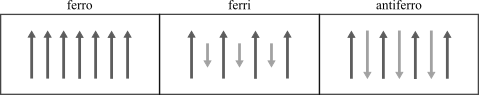
\includegraphics[width=\textwidth]{pictures/magnetic_order.png}
    \caption{Schematic depiction magnetically ordered materials.}
    \label{fig:magnetic_order}
\end{figure}
\FloatBarrier 


\subsection{Domains}
To understand the origin of ultrafast dynamics in magnetically ordered systems we first need to understand what domains are.
They are defined as regions of uniform direction of the order parameter, in the case of ferromagnets it is the magnetization.
This splitting of the magnetic structure into different domains is caused by the minimization of the free energy in the material.
There are several energy contributions coming into play.
Only when they balance out eachother, a stable magnetic state of the sample is possible.
The first and foremost term involved in the forming of domains is the field energy $E_{\text{f}}$ stored in form of the magnetostatic field around the sample.
A large domain also generates a large magnetic field as the field energy scales with the square of the domain size.
Therefore to reduce the field energy the material is split into domains of ever smaller size.
But this shrinking of the domain sizes does not go on indefinetely.
One of the opposing energy terms is the domain wall energy $E_{\text{D}}$ and scales with the root of the domain size.
At the boundries between different domains, which are called domain walls, neighbouring magnetic moments are forced to point in opposite directions.
This goes against the exchange interaction trying to align the magnetic moments in the same direction and there is a energy cost associated with it.
So the domain size is mostly determined by the balance of the field energy saved by domain splitting and the energy cost of additional domain walls.

A further reduction of the field energy is brought on by neighbouring domains having orthogonal magnetizations.
The involved domains are then called flux closure domains.
As the name implies trough the orthogonal arrangement of the domains the field loops get closed almost entirely inside the material.
Since magnetic media have an easy direction of magnetization, flux closure domains result in the magnetization of some domains to be at an angle to this easy direction.
This introduces two additional energetic costs to the equation.
Having the orientation of magnetization at an angle to the easy axis causes an energy term, the magnetocrystalline anisotropy energy $E_{\text{mc}}$, to arise as it is more energetically favourable to have the magnetic moments to align parallel to the easy axis.
The magnetoelastic anisotropy energy $E_{\text{me}}$ is another term caused by a deviation of the orientation of magnetization from the easy axis.
% As a consequence the magnetic dipoles, meaning the ions, deform slightly which induces tiny mechanical stresses on the sample and thus the emerging of such a domain comes with an energy cost.
As a consequence the magnetic dipoles, meaning the ions, deform slightly which induces tiny mechanical stresses on the sample, leading to a phenomenon labeled magnetostriction.
This results in an energy cost hindering the emergence of such closure domains at an angle to the easy axis.

All of these odds in the form of energy costs are stacked against non-parallel alignment to the easy axis which means that most of the volume in a magnetic material holds domains with their magnetization oriented parallel to the easy direction.
This equation
\begin{equation}
    E_{\text{f}} = E_{\text{D}} + E_{\text{mc}} + E_{\text{me}}
    \label{eqn:landau_lifschitz_energy}
\end{equation}
summarizes all the different energy components involved in domain formation.

\subsection{Antiferromagnetic domains}

\section{Magnon dynamics} 


% \section{Sample system NiO/C60}
\section{NiO}
As Ni is a transition metal it carries some unique properties simplifying possible theoretical calculations and making it especially interesting for fundamental research of magnetic materials.
The electronic structure of Ni is $[\text{Ar}]3$d$^8 4$s$^2$.
Entering into a covalent bond with the oxygen 2p-ions the electron configuration of Ni$^{2+}$ changes to $[\text{Ar}]3$d$^8$.
Having a partially filled 3d-orbital in its electronic structure each Ni-ion possesses a net magnetic moment, caused by the angular momenta associated with the unpaired electrons.
Both the orbital angular momentum and the spin of an electron create a magnetic moment.
For a multielectron ion such as Ni$^2+$ with a relatively weak spin-orbit coupling all the angular momenta of each electron couple via the Russel-Saunders coupling.
A big difference to other classes of magnetically ordered elements such as rare earths and actinides is the spatial position of those partially filled shells.
As our object of interest are not single atoms, but crystals containing them, the interaction of the electrostatic crystal field with the orbital motion of the electron is not to be dissmissed.

Rare earths and actinides having their partially filled orbitals (4f and 5f) screened by outer lying shells experience the crystal field interaction as relatively weak or rather just as a small perturbation \lit{Tanner, B. K. (1979)}.
Whereas the transition metals outermost orbitals are exactly those unfilled 3d-shells exposed to the crystal field.
Here, the crystal field is strong in comparison to the spin-orbit interaction.
This leads to their orbital angular momentum being quenched, so that only the magnetic moments of the spin attributes to the net magnetic moment of the ions.

In terms of energy levels the octahedral crystal field exerted by the six neighbouring O$^{2-}$ is responsible for the splitting of the d-states $\Delta_{\text{CF}}$ by lifting the degeneracy in the magnetic quantum number $m_l$.
Additionally an exchange splitting $\Delta_{\text{Ex}}$ takes place depending on the orientation of the spins.
If the exchange splitting is bigger than the crystal-field splitting $\Delta_{\text{Ex}} > \Delta_{\text{CF}}$, as for example in MnO, the spins occupy the lowest possible states, which results in a high-spin state, as seen in \autoref{fig:2}a).
In NiO the exchange and crystal splitting are of similar size and the electrons would occupy a high-spin state as shown in \autoref{fig:2}b) with $S=1$. But even in the case that $\Delta_{\text{CF}}$ would slightly exceed $\Delta_{\text{Ex}}$ the d$^8$-electrons would occupy the same ground state.
Given, the order of the filling would change but the end result would still be the same as with $\Delta_{\text{Ex}} > \Delta_{\text{CF}}$, because the t$_{\text{2g}}$-orbital can contain three electrons and the e$_{\text{g}}$-orbital can contain two electron there is no other way for the d$^8$-electrons to order.
\begin{figure}[ht]
    \centering
    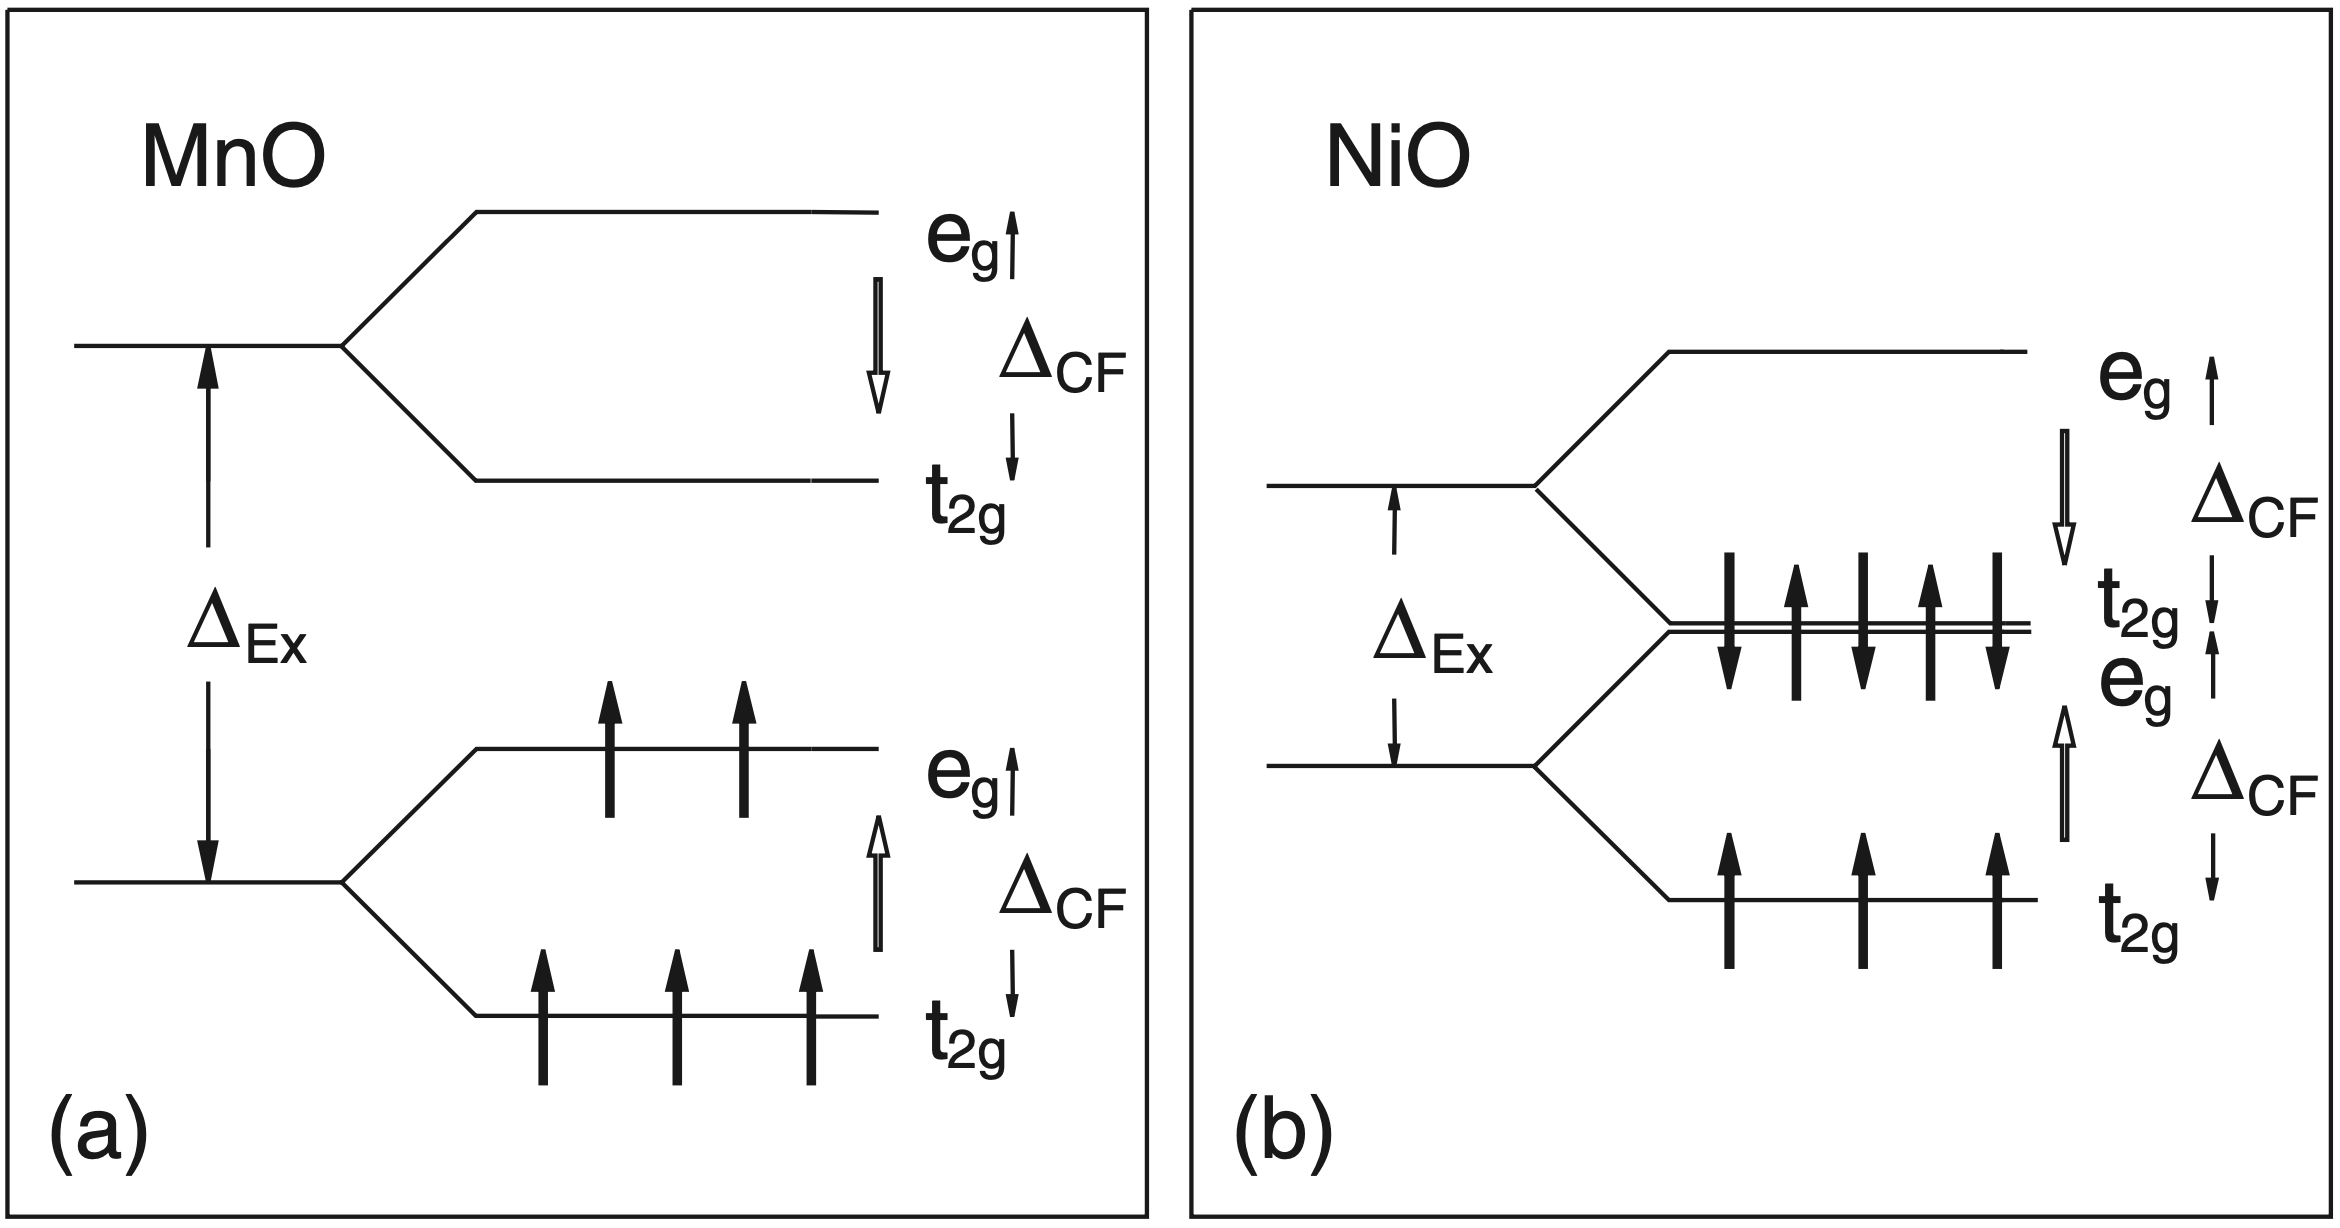
\includegraphics[width=0.8\textwidth]{pictures/2.png}
    \caption{Schema of energy levels of \textbf{(a)} MnO and \textbf{(b)} NiO split by the exchange interaction and by the crystal field. Taken from \lit{B. Fromme}}
    \label{fig:2}
\end{figure}
\FloatBarrier
The one-electron picture including only the Coulomb interactions makes for an intuitive understanding of the occupancy of the ground state, but it does not give the right sizes of the splitting.
The multi-electron picture taking into account the covalency of the 3d-electrons and the 2p-electrons from the oxygen ions and the overlap of the wavefunctions by using the Russel-Saunders terms instead of single electron states.
As the spin-orbit interaction is small the LS-coupling is dominant summing up the angular momenta of each electron s, p, d, ... to the total angular momenta of the whole Ni$^{2-}$-ion S, P, D, ... according to the Hund's rules.
Now the effect of the crystal field on the Russel-Saunders split energy levels of the transition metal ion is calculated.
The crystal field strength $Dq/B$ is taken as a parameter and factors in the Coulomb and also the covalent interaction between the Ni- and O-ions.
Plotting the energy levels against the crystal field strength gives the so called Sugano-Tanabe-diagrams \autoref{fig:4}, which can then be aligned to an absorption spectrum to extract a rough estimate for the crystal field strength, but more importantly to assign experimental results such as absorption edges or transition to the right multiplets.
The result of such an approach is depicted in \autoref{fig:3}.

\begin{figure}[ht]
    \centering
    \begin{subfigure}[b]{0.4\textwidth}
        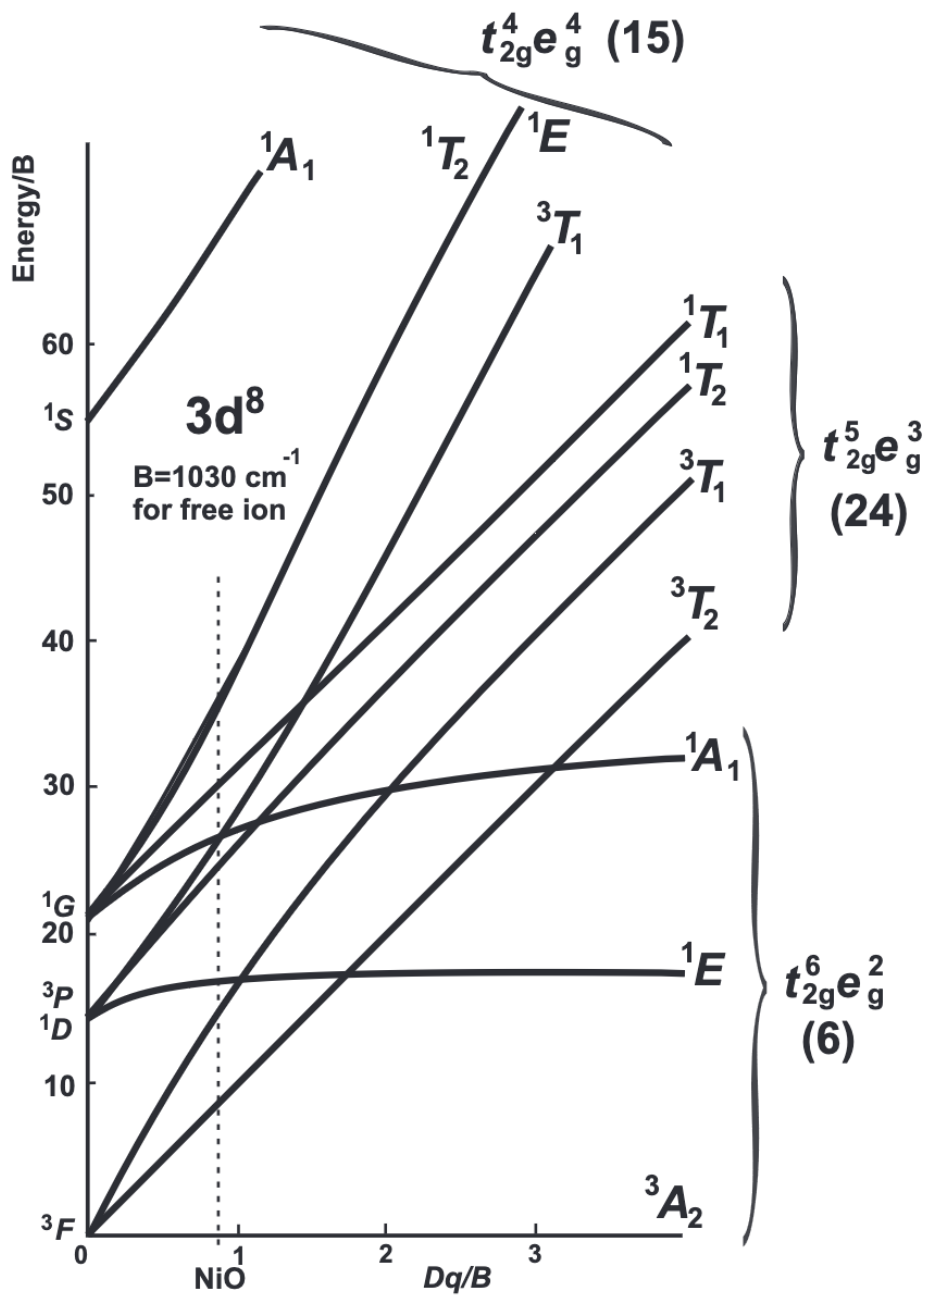
\includegraphics[width=\textwidth]{pictures/4.png}
        \caption{}
        \label{fig:4}
    \end{subfigure}
    \hspace{1cm}
    \begin{subfigure}[b]{0.4\textwidth}
        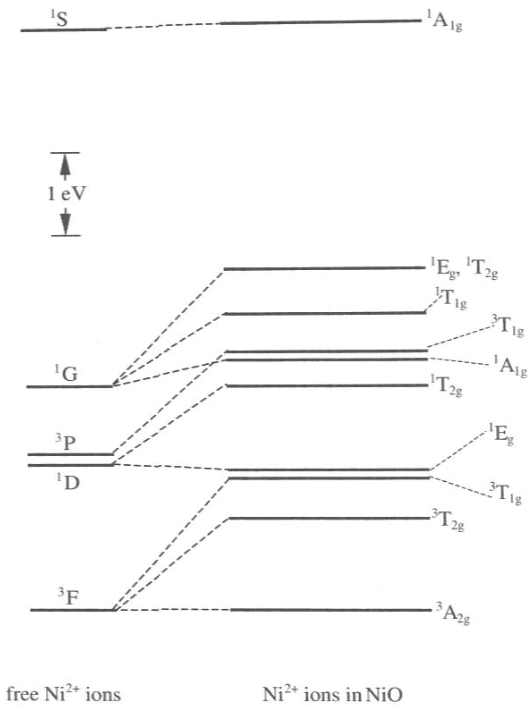
\includegraphics[width=\textwidth]{pictures/3.png}
        \caption{}
        \label{fig:3}
    \end{subfigure}
    \caption{\textbf{a)} The Sugano-Tanabe diagram for Ni$^{2+}$-ions, where the energy levels are plotted against the crystal field strength $Dq/B$. \textbf{b)} The Russel-Saunders terms of the free Ni$^{2+}$-ions on the left and the crystal field splitting of the Ni$^{2+}$-ions in an octahedral field in NiO on the right. Taken from \lit{B. Fromme}}
\end{figure}
\FloatBarrier



\subsection{Magnetic structure}
As mentioned above, the driving force behind the AFM order is the superaxchange between two Ni-ions which are positioned on opposite sites of an O-ion.
In \autoref{fig:1}b its clearly visible that the AFM coupling occurs in one of the $\langle100\rangle$-directions.
The cubic rocksalt structure of the NiO in the paramagnetic phase becomes a rhombohedral one, when going beneath the Neél-temperature of $T_N = \qty{523}{K}$ as the AFM order induces a slight contraction along one of the four equivalent $\langle111\rangle$-axes.
As a result the optic axis also forms along this direction.
In its ordered phase NiO has a cubic anisotropy, meaning two anisotropy directions.
One is the hard axis, where all the atomic spins lie in ferromagnetic sheets in the $(111)$-plane, making it a prototypical easy-plane antiferromagnet.
The magnetization in neighbouring sheets is reversed.
The second one is the easy axis and although it was under some discussion, the consensus now is \lit{Hutchings and Samuelsen; Roth et al.} that the spins point in the $\langle11\overline{2}\rangle$-direction.

Because the rhombohedral contraction can happen along any one of the four equivalent $\langle111\rangle$-axes there exist four twin- or T-domains.
Within these T-domains there are further three equivalent $\langle11\overline{2}\rangle$-axes to which the spins can lie parallel.
These regions of the same spin orientations within the FM sheets are called S-domains, making it a total of 12 possible domains.
Domains can also originate from structural defects, as the strystal structure is tightly connected to the magnetic structure.
Nonetheless, the existence of these domains plays a key role in making the excitation of both magnon modes in NiO possible.
\begin{figure}[ht]
    \centering
    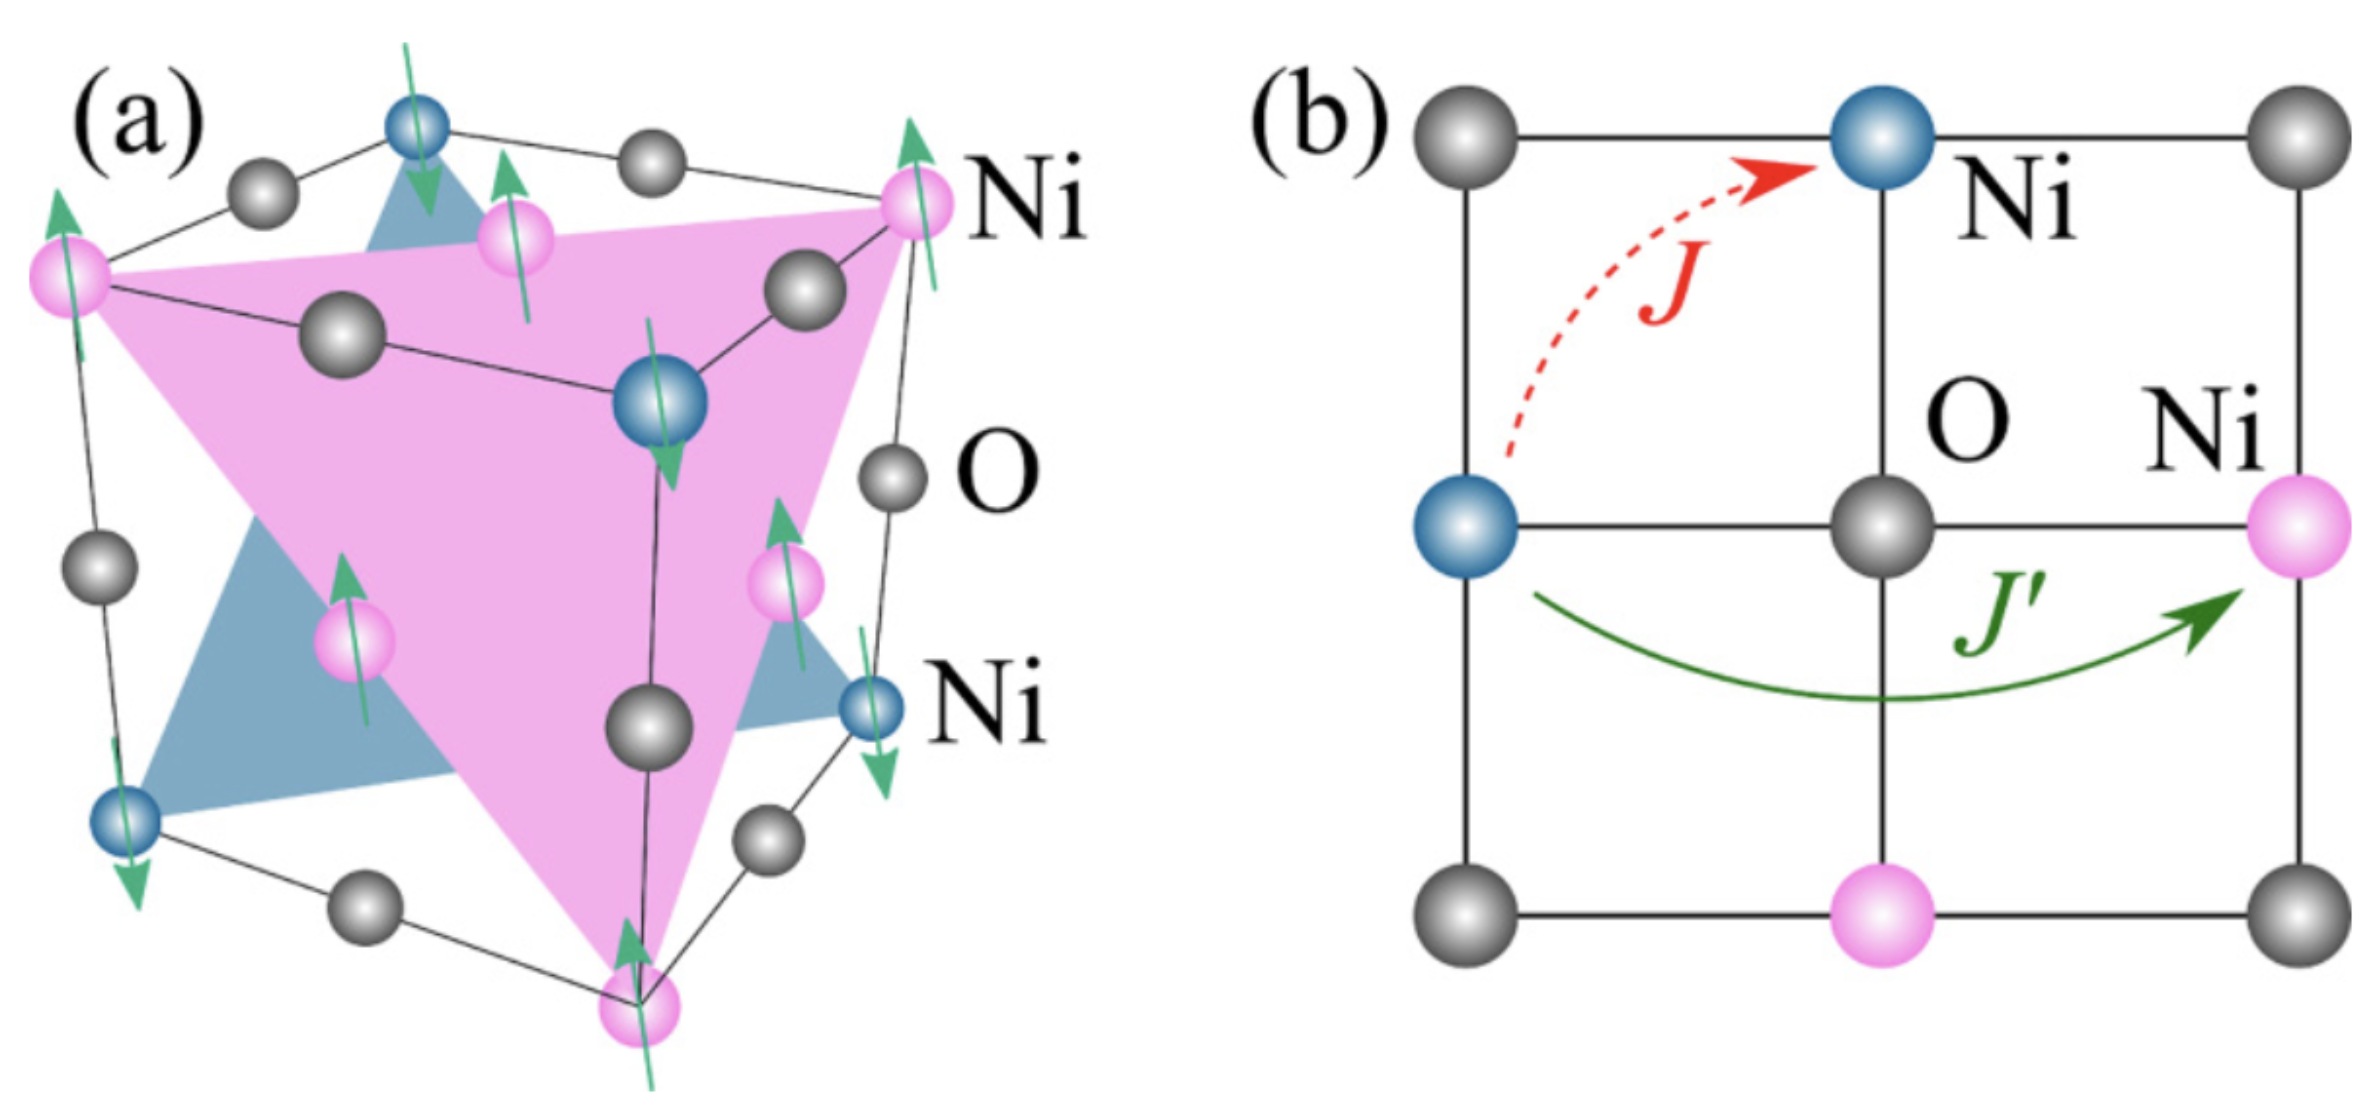
\includegraphics[width=0.6\textwidth]{pictures/1.png}
    \caption{A representation of the crystal and magnetic structure of NiO. Taken from \lit{Betto et al.}}
    \label{fig:1}
\end{figure}
\FloatBarrier

\subsection{Exciton-Magnon-Transition}
Many absorption spectra of antiferromagnetic insulators exhibit an additional peak right next to their exciton peaks \lit{Sell} refered to as magnon sideband.
We utilize this exciton-magnon transition to create magnons in NiO.
The exciton peak visible in the absorption spectrum of NiO \autoref{fig:5} at around \qty{0.97}{eV} originates from the spin-forbidden electric dipole d-d transition between the crystal field multiplets $^3A_{2g} \rightarrow \, ^3T_{2g}$.
All d-d transitions in centrosymmetric environments, such as the octahedral one of the Ni$^{2+}$-ions, are parity forbidden by the Laport rule $\Delta L = \pm 1$.
This selection rule is easily explained when you consider the symmetry of the the initial wavefunction $\Psi_i$, the final wavefunction $\Psi_f$ and the transition moment operator $\mu$, when looking at the transition matrix element
\begin{equation}
    M_{if} = \int_{\mathbb{R}^3} \Psi^*_f \cdot \mu \cdot \Psi_i \;\text{d}r^3 \;.
    \label{eqn:laport}
\end{equation}
For the matrix element to be non-zero when integrating over the whole euclidian space the product $\Psi^*_f \cdot \mu \cdot \Psi_i$ inside the integral in \autoref{eqn:laport} has to have an even parity.
For electric dipole transitions the $\mu$ is odd, so that a transition is only allowed if the initial and final wavefunction are of different parities totaling to an odd parity.
What breaks the inversion symmetry in NiO and what allows for the d-d transition to happen is the silmultaneous creation of a magnon.
For an intuitive understanding you could think of this in the same way as thinking of a phonon with an odd vibration breaking the centrosymmetry and thus allowing d-d transitions showing itself as a phonon sideband.
The spin-forbideness is also lifted by the magnon as it compensates the spin, which is only possible and also why we only see this in antiferromagnets.
\begin{figure}[ht]
    \centering
    \begin{subfigure}[b]{0.3\textwidth}
        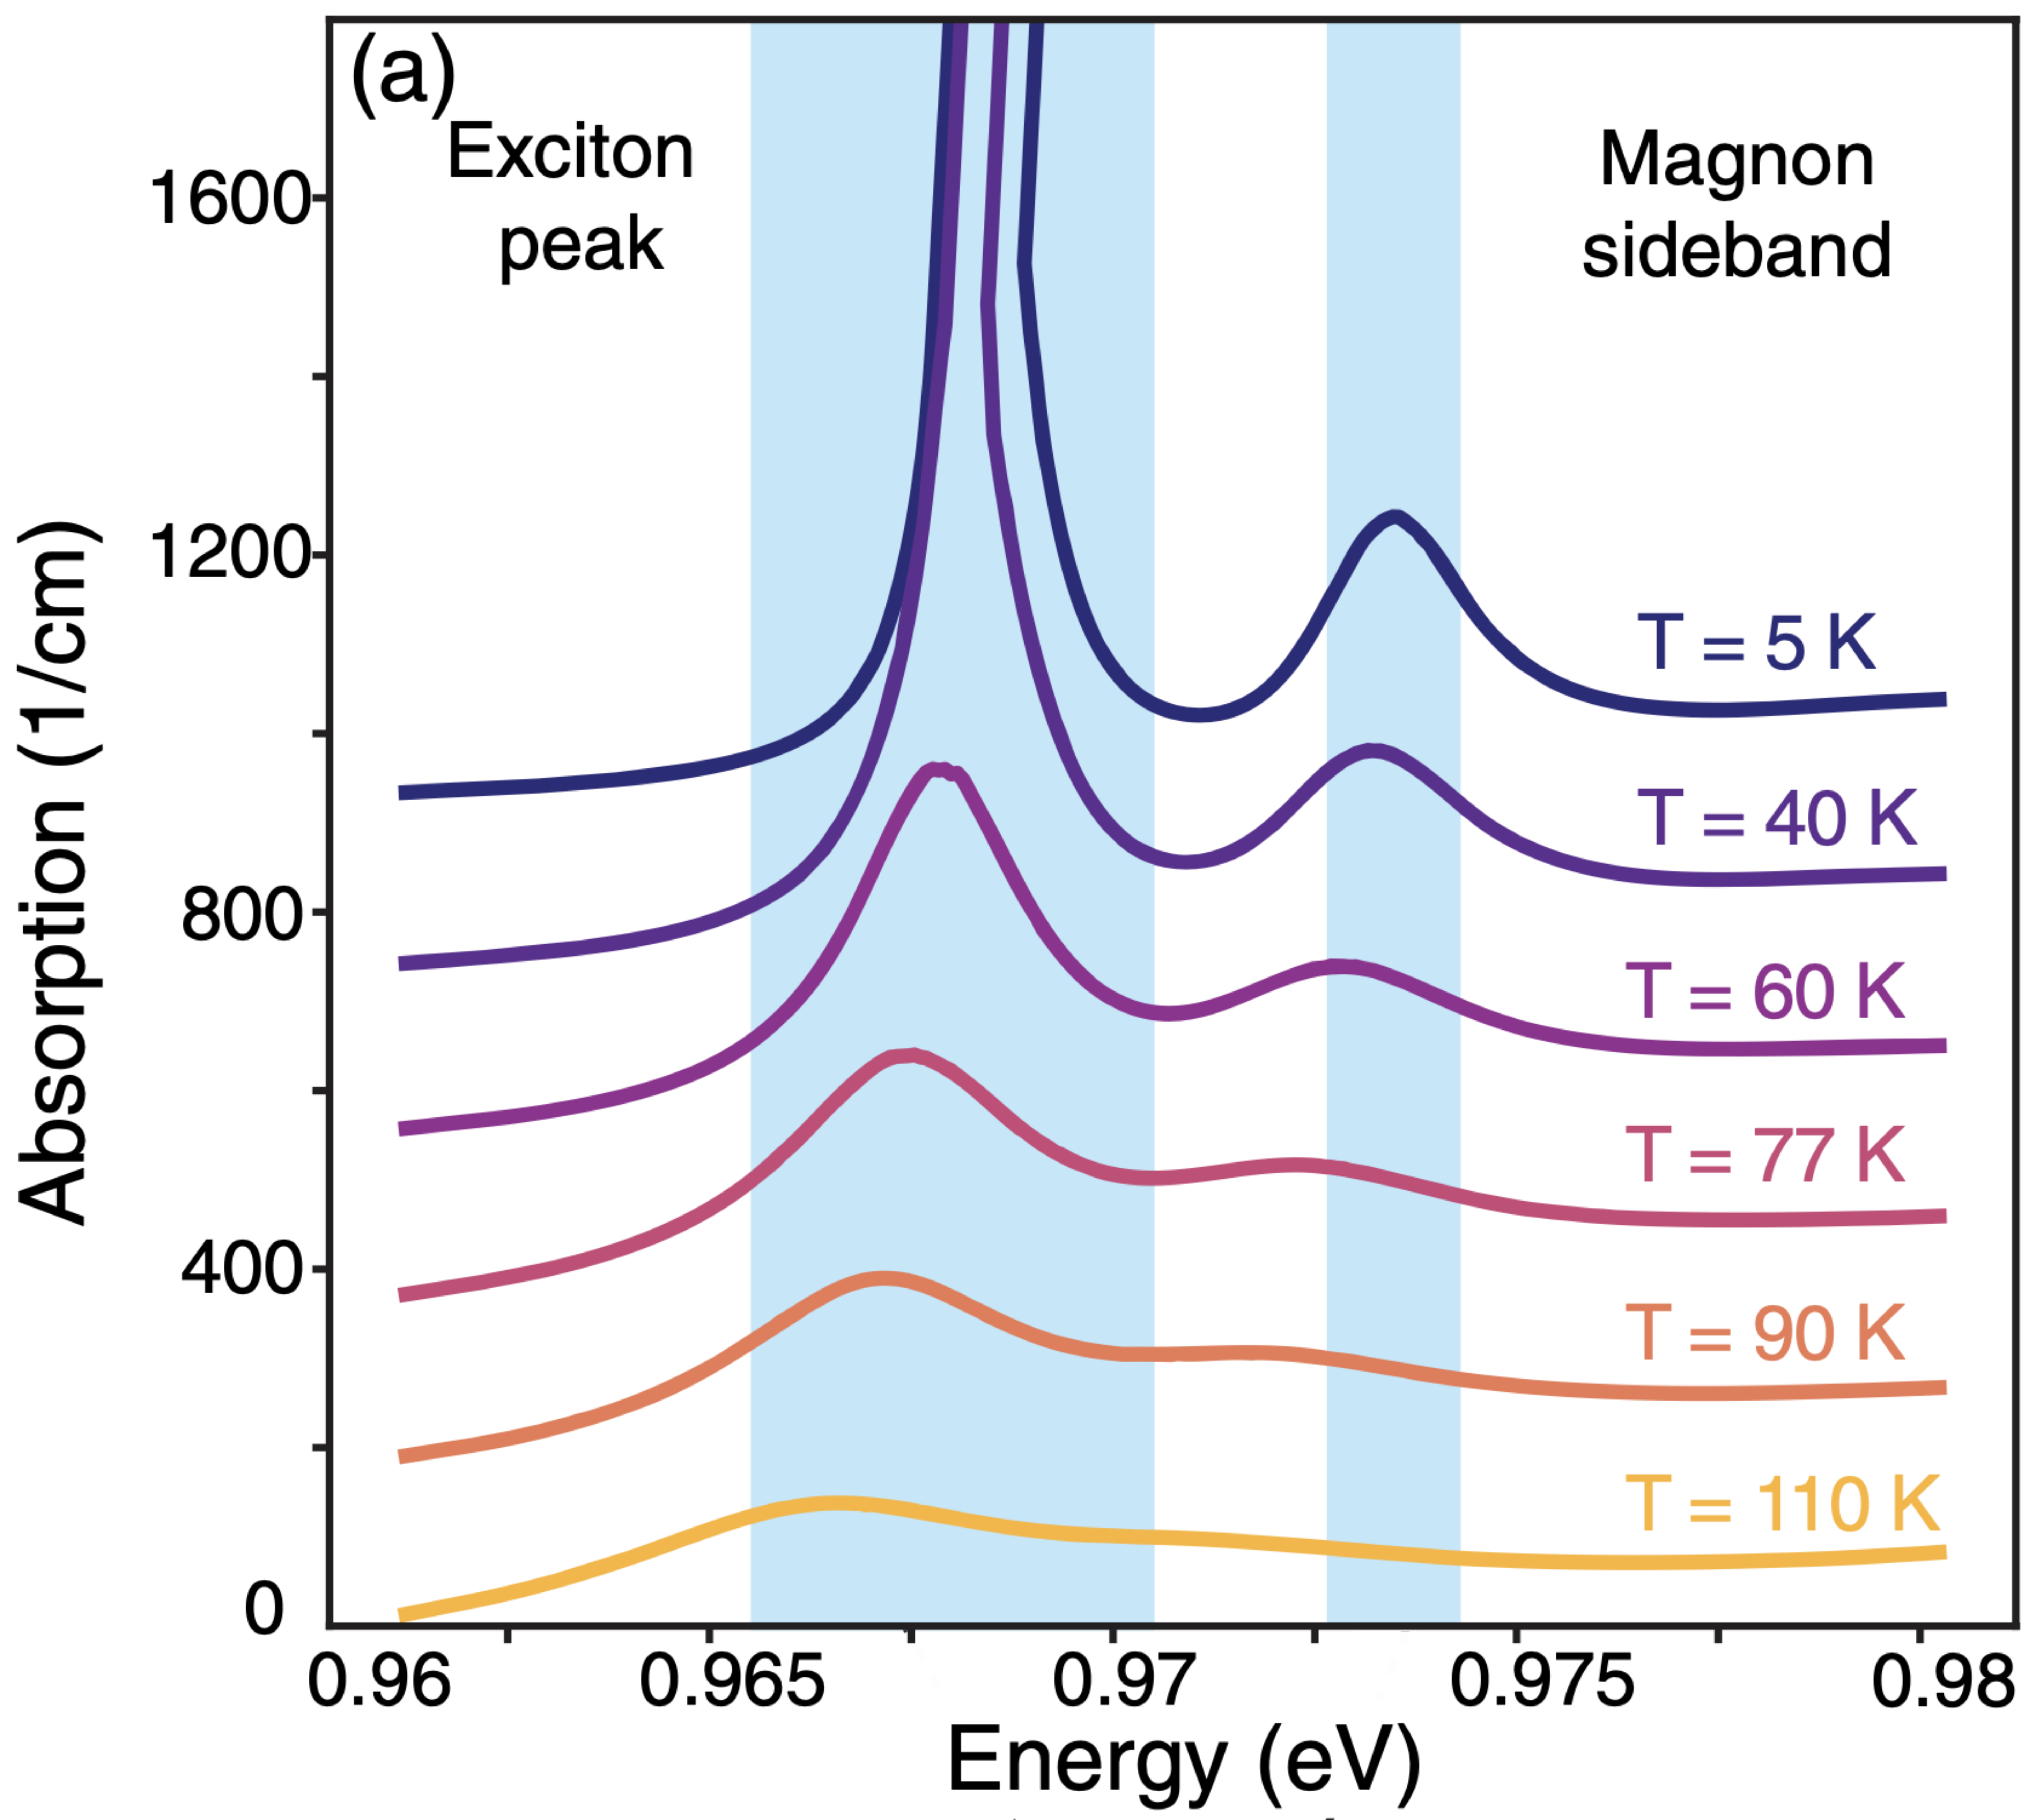
\includegraphics[width=\textwidth]{pictures/5.png}
        \caption{}
        \label{fig:5}
    \end{subfigure}
    \hspace{1cm}
    \begin{subfigure}[b]{0.6\textwidth}
        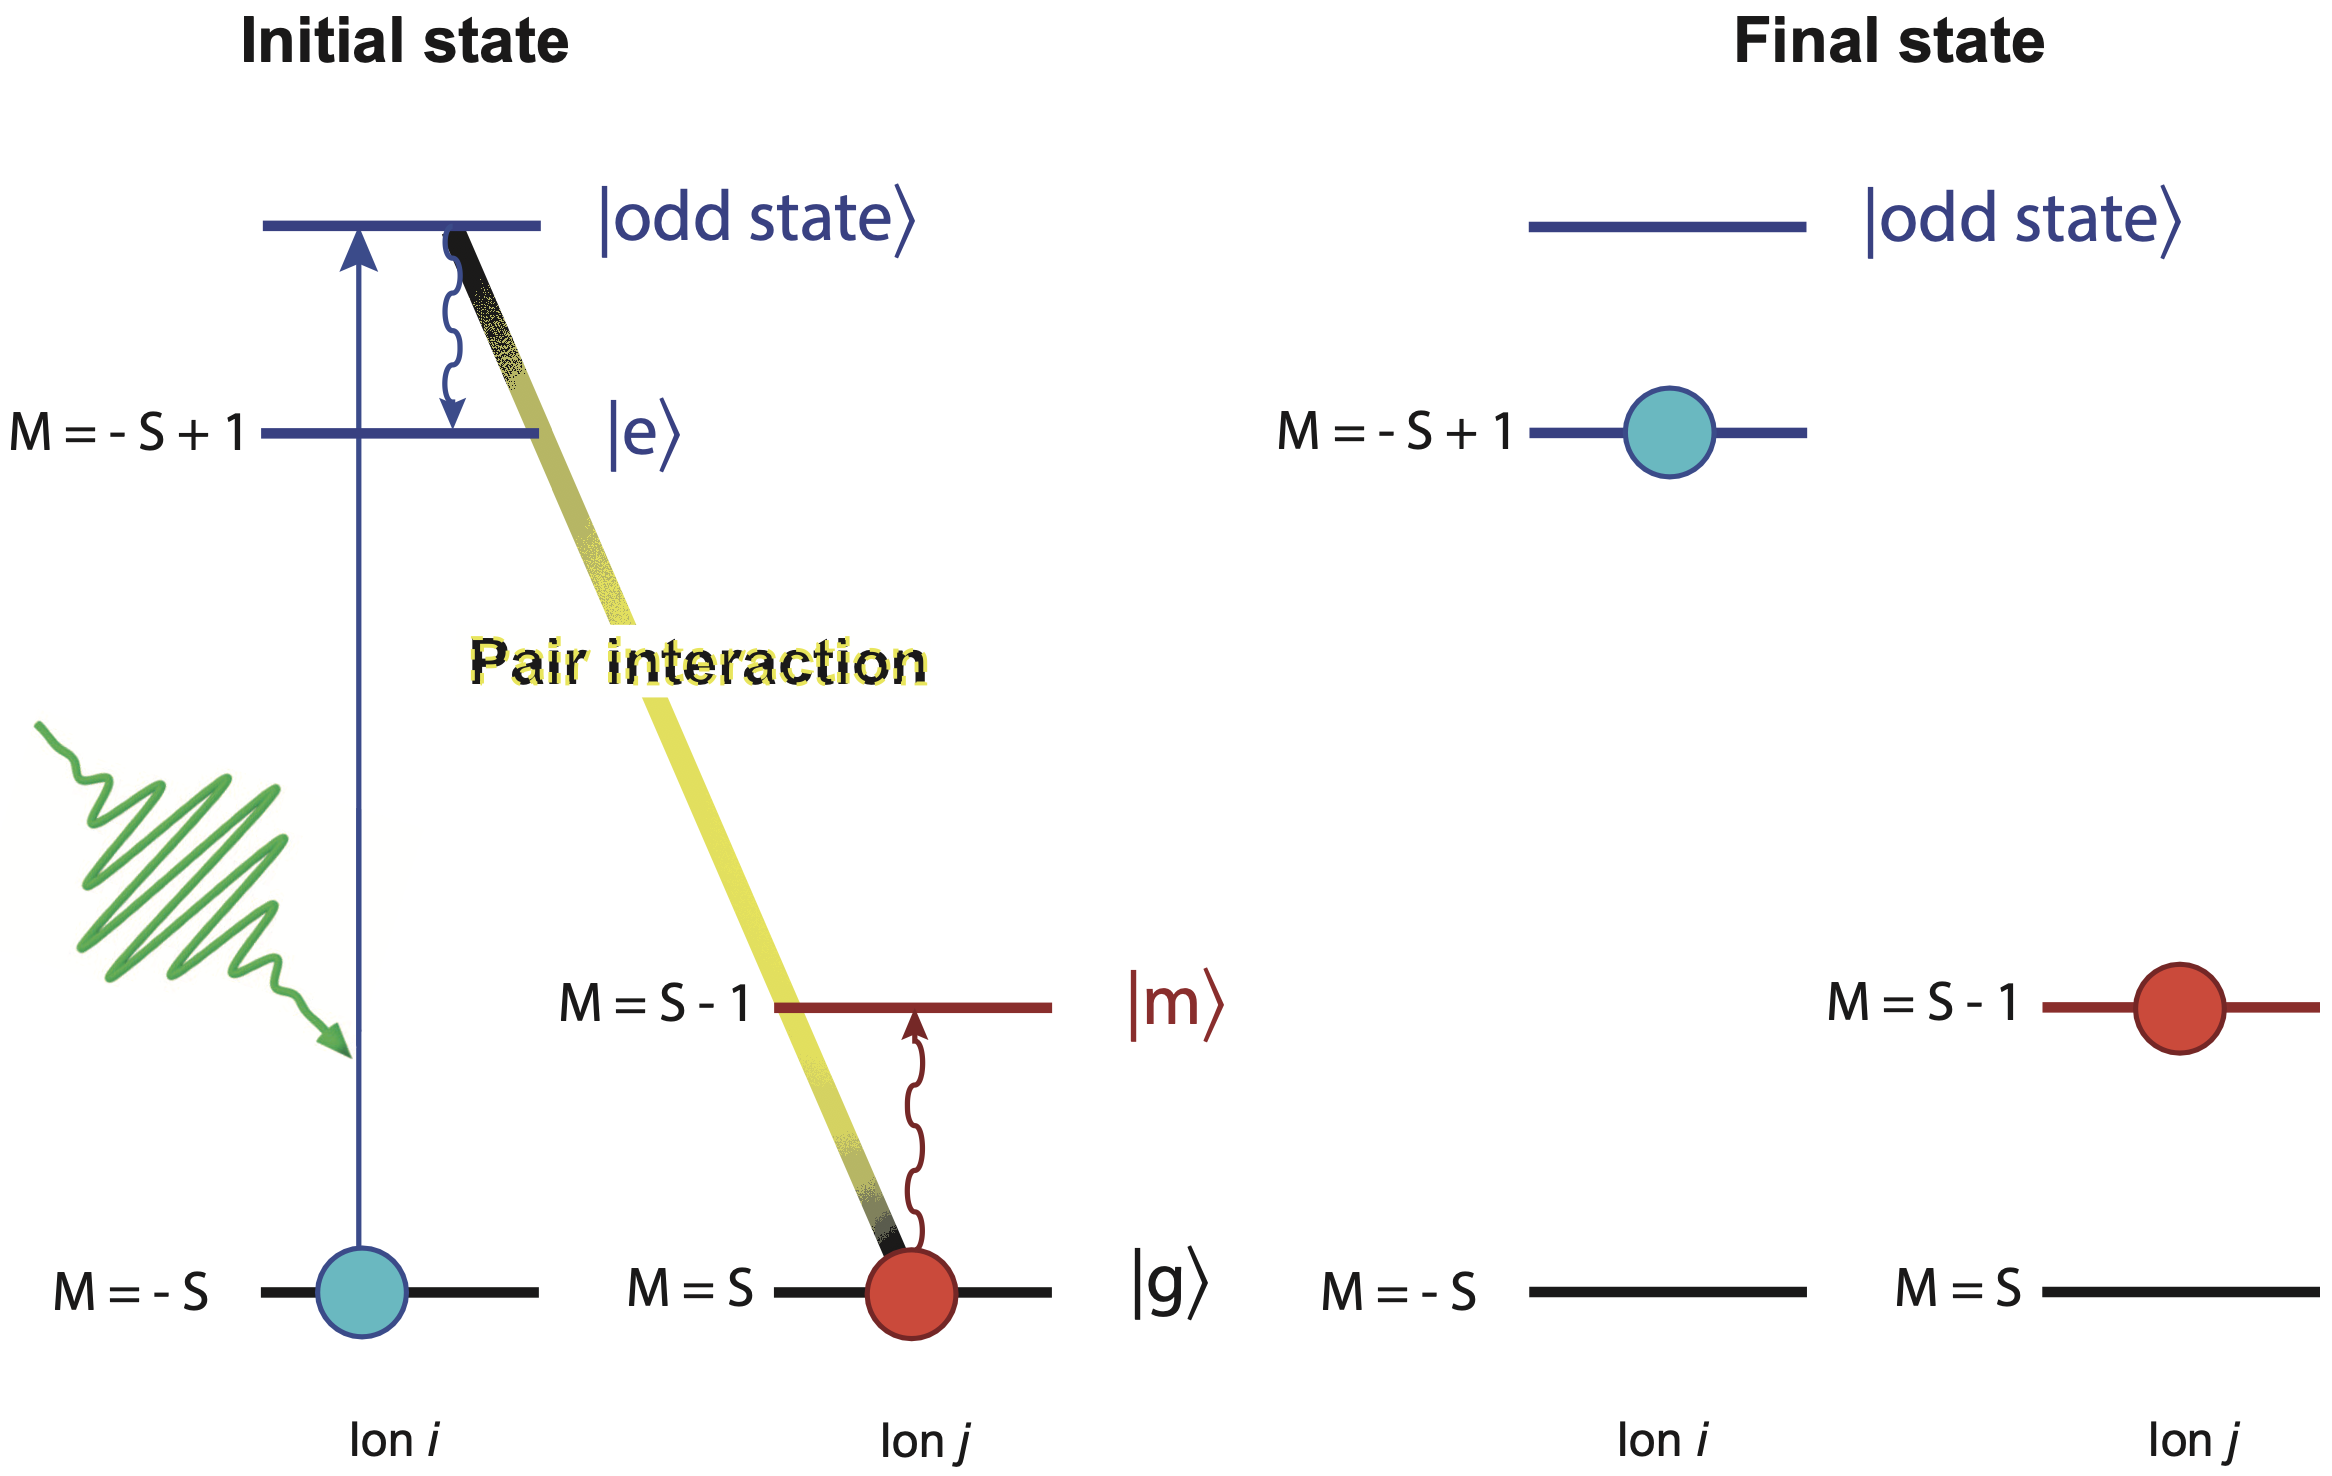
\includegraphics[width=\textwidth]{pictures/6.png}
        \caption{}
        \label{fig:6}
    \end{subfigure}
    \caption{\textbf{a)} The absorption of NiO in the energy range around the exciton-magnon resonance, measured at different temperatures. \textbf{b)} A schematic representation of the energy levels and transitions involved in the exciton-magnon transition. Taken from \lit{Bossini et al.}}
\end{figure}
\FloatBarrier
\autoref{fig:6} shows a schematic diagram on the basis of which the explanation of the concrete process behind the exciton-magnon transition is easier to follow.
Two Ni$^{2+}$-ions, each from one of the two sublattices, are involved in this scheme.
First, a photon hits the 1. ion with spin $-S$ and raises it into an opposite parity state compared to the ground state, which is odd since the ground state is taken as even.
This electron excitation is described as a Frenkel exciton, because the spatial extensions of the involved d-orbital are small compared to the lattice parameter, which is exactly the case for the tightly bound 3d-electron in the Ni-ions.
The ion relaxes to its final state $|e\rangle$ with even parity, but undergoing a change in spin to $-S+1$.
Silmultaneously, mediated by the superexchange interaction between the two ions, the 2. ion in the other sublattice with spin $S$ undergoes an electric-dipole transition to a state $|m\rangle$ with spin $S-1$.
These two spin-changing transitions are only possible, because they happen at the same time and the total spin is conserved.
Frenkel excitons with a change of spin are essentially spin waves, so this whole process effectively created a magnon mode causing the precession of spins in both sublattices.

\subsection{Magnon coupling}
Theory predicts different AFM resonance modes depending on the model used to simulate the dispersion and magnetic or temperature dependencies.
They contain different interactions and different amounts of sublattices.
A two-lattice model is best used to describe the two magnon modes at the Brioullin-zone center with frequencies of \qty{1.07}{THz} and \qty{0.13}{THz} visible when pumping with light in the infrared region.
Apparently
There is also a 8-sublattice model predicting five different degenerate modes at $k=0$ 

\section{C60}




